\documentclass[14pt, a4paper]{report}
\usepackage{mathtext}
\usepackage[T2A]{fontenc}
\usepackage[utf8]{inputenc}
\usepackage[russian]{babel}
\usepackage{multirow}
\usepackage{slashbox}
\usepackage{makecell}
\usepackage{graphicx}
\usepackage{physics}
\usepackage{amstext}
\usepackage{caption}
\usepackage{subcaption}
\usepackage{cmap}
\usepackage{float}
\usepackage{indentfirst}
\usepackage{romannum}

\usepackage[a4paper,
            		left=1in,
            		right=1in,
           		 top=1in,
            		bottom=1in,
            		footskip=.25in]{geometry}

\renewcommand{\thesection}{\arabic{section}.}
\renewcommand{\thesubsection}{\arabic{section}.\arabic{subsection}.}

\title{\textbf{Отчет о выполнении лабораторной работы 1.2 "Исследование эффекта Комптона"}}
\author{Калашников Михаил, Б03-202}
\date{}

\begin{document}
\maketitle

\pagenumbering{arabic}

\textbf{Цель работы:} Исследование энергетического спектра $\gamma$-квантов, рассеянных на графите, с помощью стинцилляционного спектромета. Определение энергии рассеянный $\gamma$-квантов в зависимости от угла рассеяния, а также энергии покоя частиц, на которых происходит комптоновское рассеяние.
\newline

\section{Теоретические сведения}

Рассмотрим элементарную теорию эффекта Комптона. Пусть на покоящийся электрон налетает $\gamma$-квант. После соударения электрон приобретает импульс, а $\gamma$-квант рассеивается на некоторый угол, по отношению к начальному направлению движения. Энергия и импульс $\gamma$-кванта также претерпят изменения. Решая систему уравнений законов сохранения энергии и импульса, получим:

\[\Delta\lambda=\frac{h}{mc}(1-\cos{\theta})\]

Основной целью лабораторной работы является проверка данного соотношения.

\section{Экспериментальная установка}

Блок схема установки изображена на рисунке ниже. Источником излучения служит $^{137}Cs$. Сформированный коллиматором узкий пучок $\gamma$-квантов попадает на графитовую мишень. Кванты, испытавшие комптоновское рассеяние в мишени, регистируются сцинтилляционным счетчиком.

\begin{figure}[H]
\centering
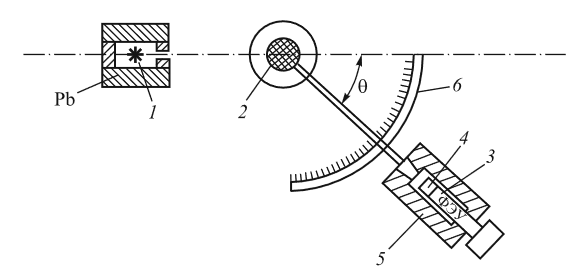
\includegraphics[scale=0.8]{../images/512-1}
\caption{Блок схема установки по изучению рассеяния $\gamma$-квантов}
\end{figure}

\section{Проведение эксперимента}

\begin{enumerate}

\item Включим все измерительные устройства и компьютер.

\item Запустим программу и войдем в режим измерения спектра.

\item Снимем спектр под различными углами в диапазоне от $0^\circ$ до $120^\circ$ с шагом $10^\circ$.

\newpage

\begin{figure}[H]
\centering
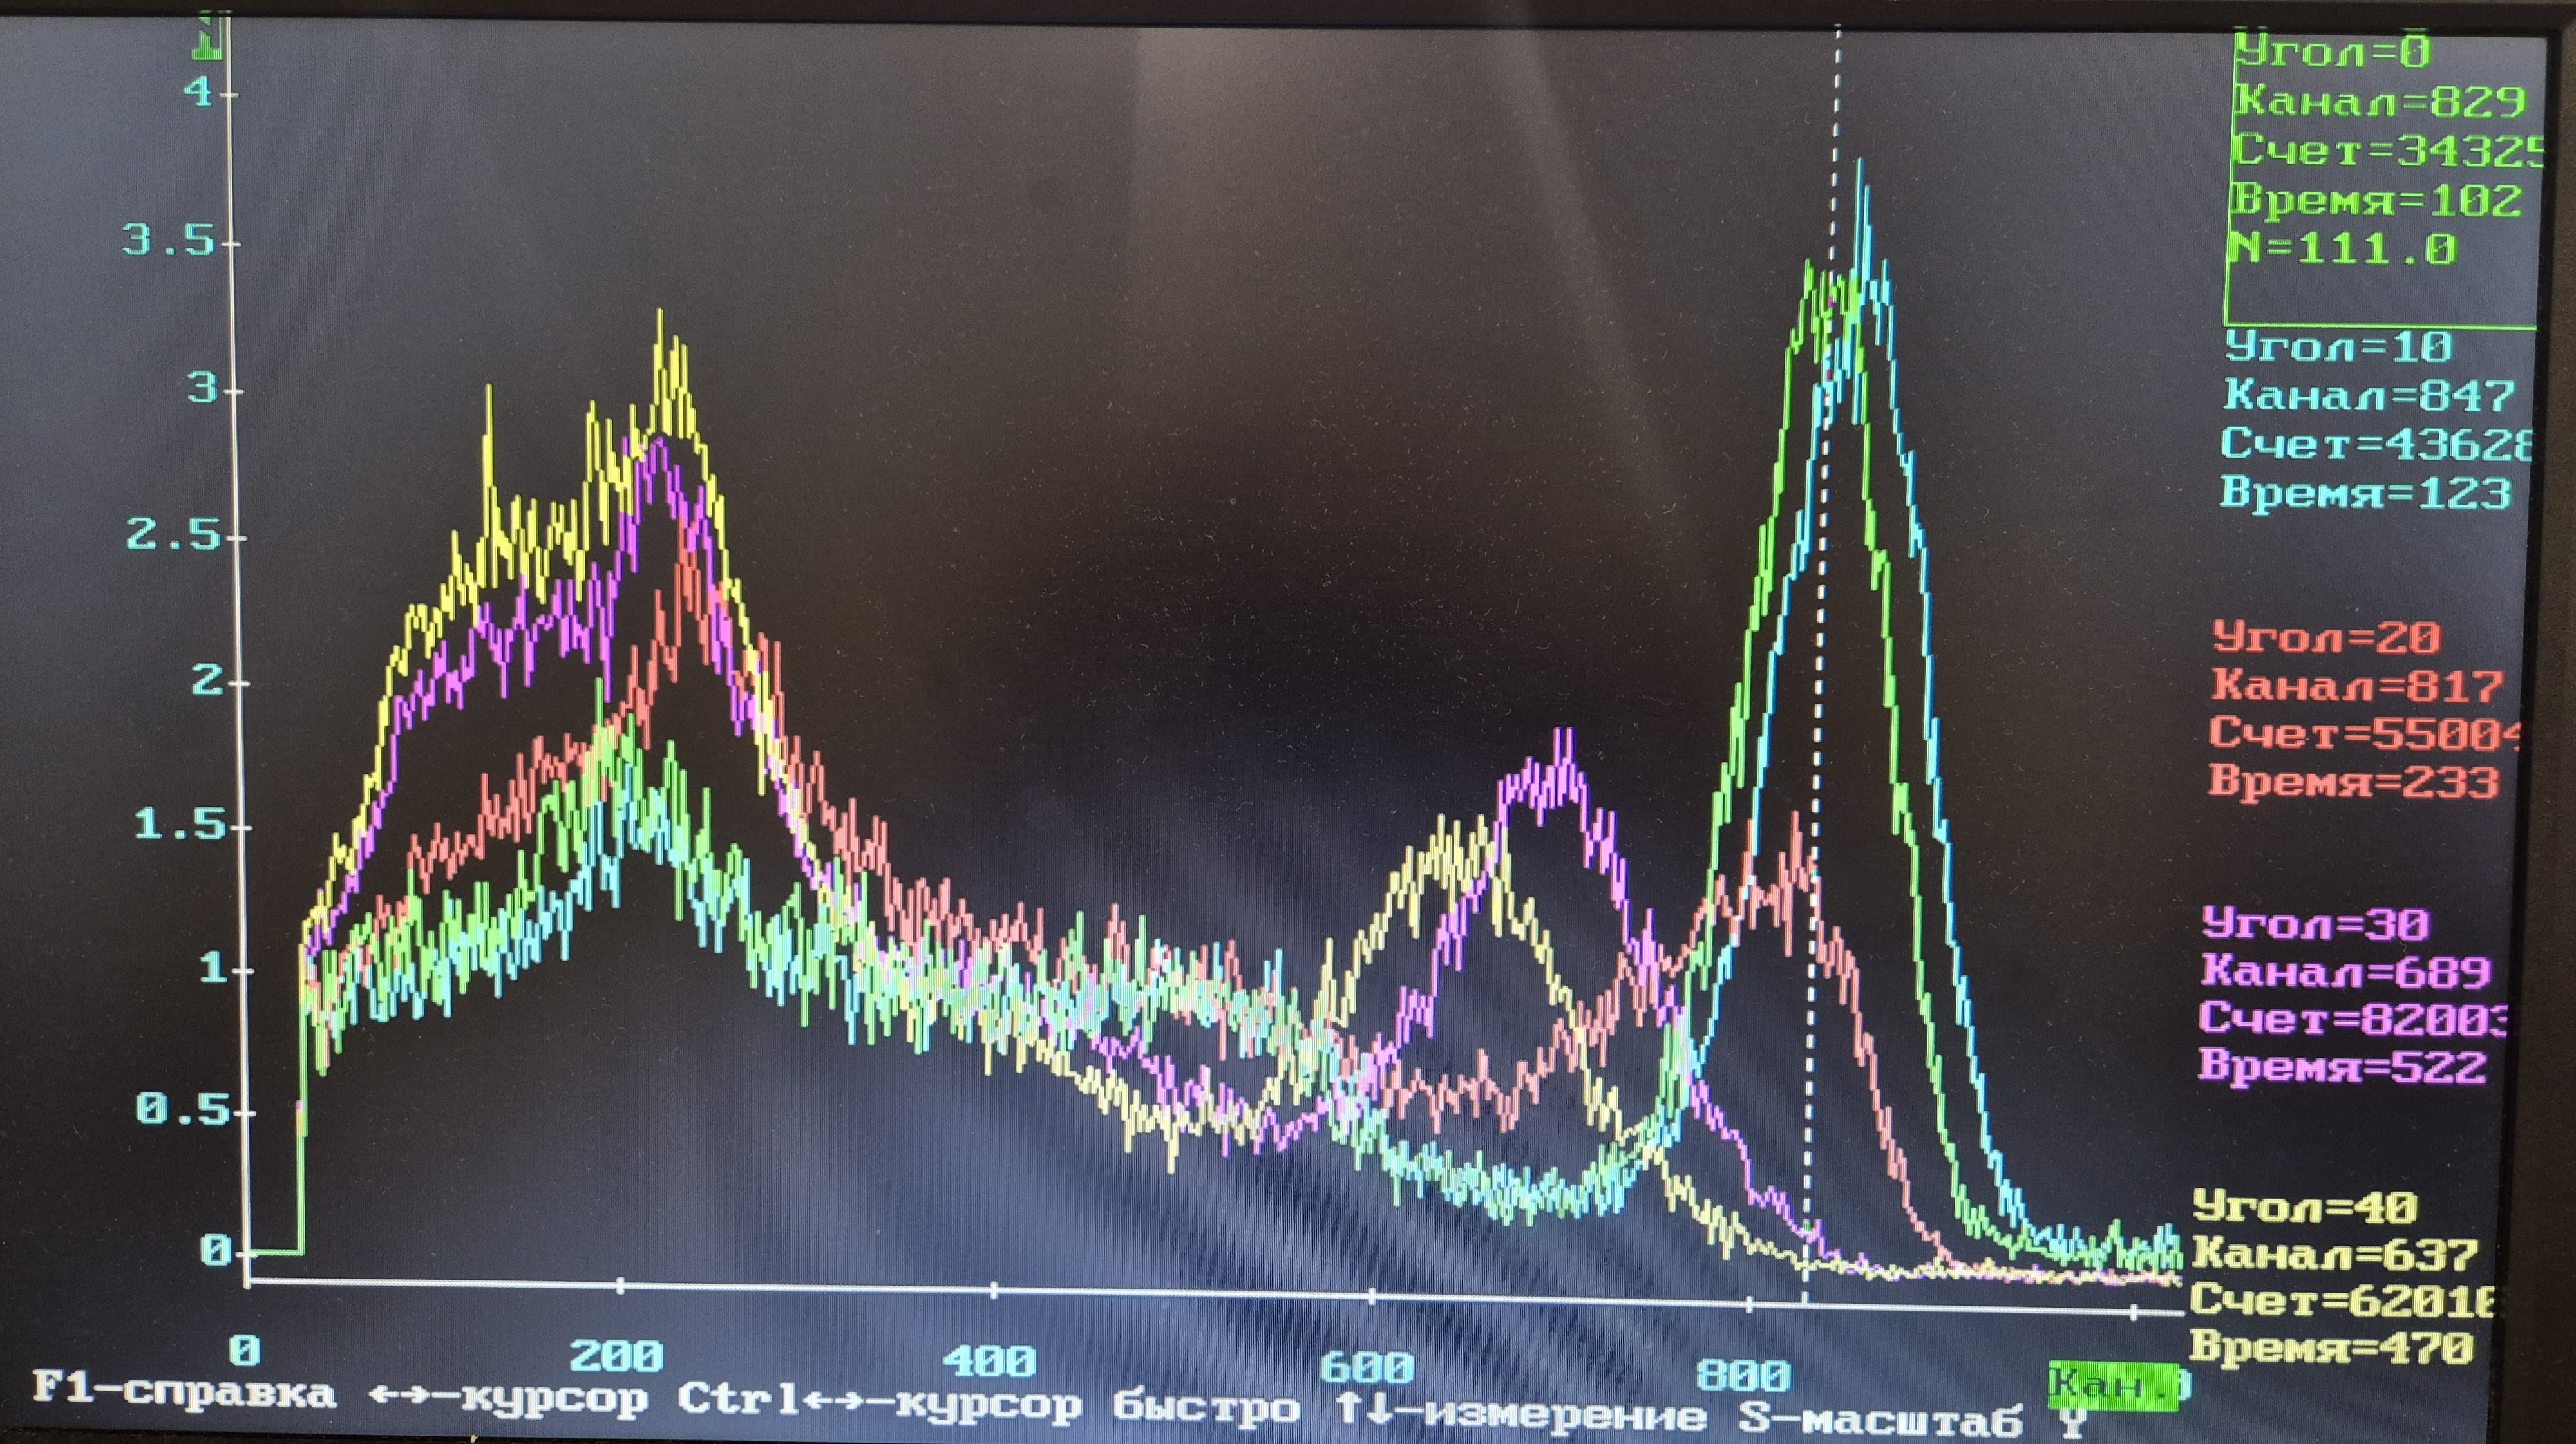
\includegraphics[width=0.85\linewidth]{../images/512-3}
\end{figure}

\begin{figure}[H]
\centering
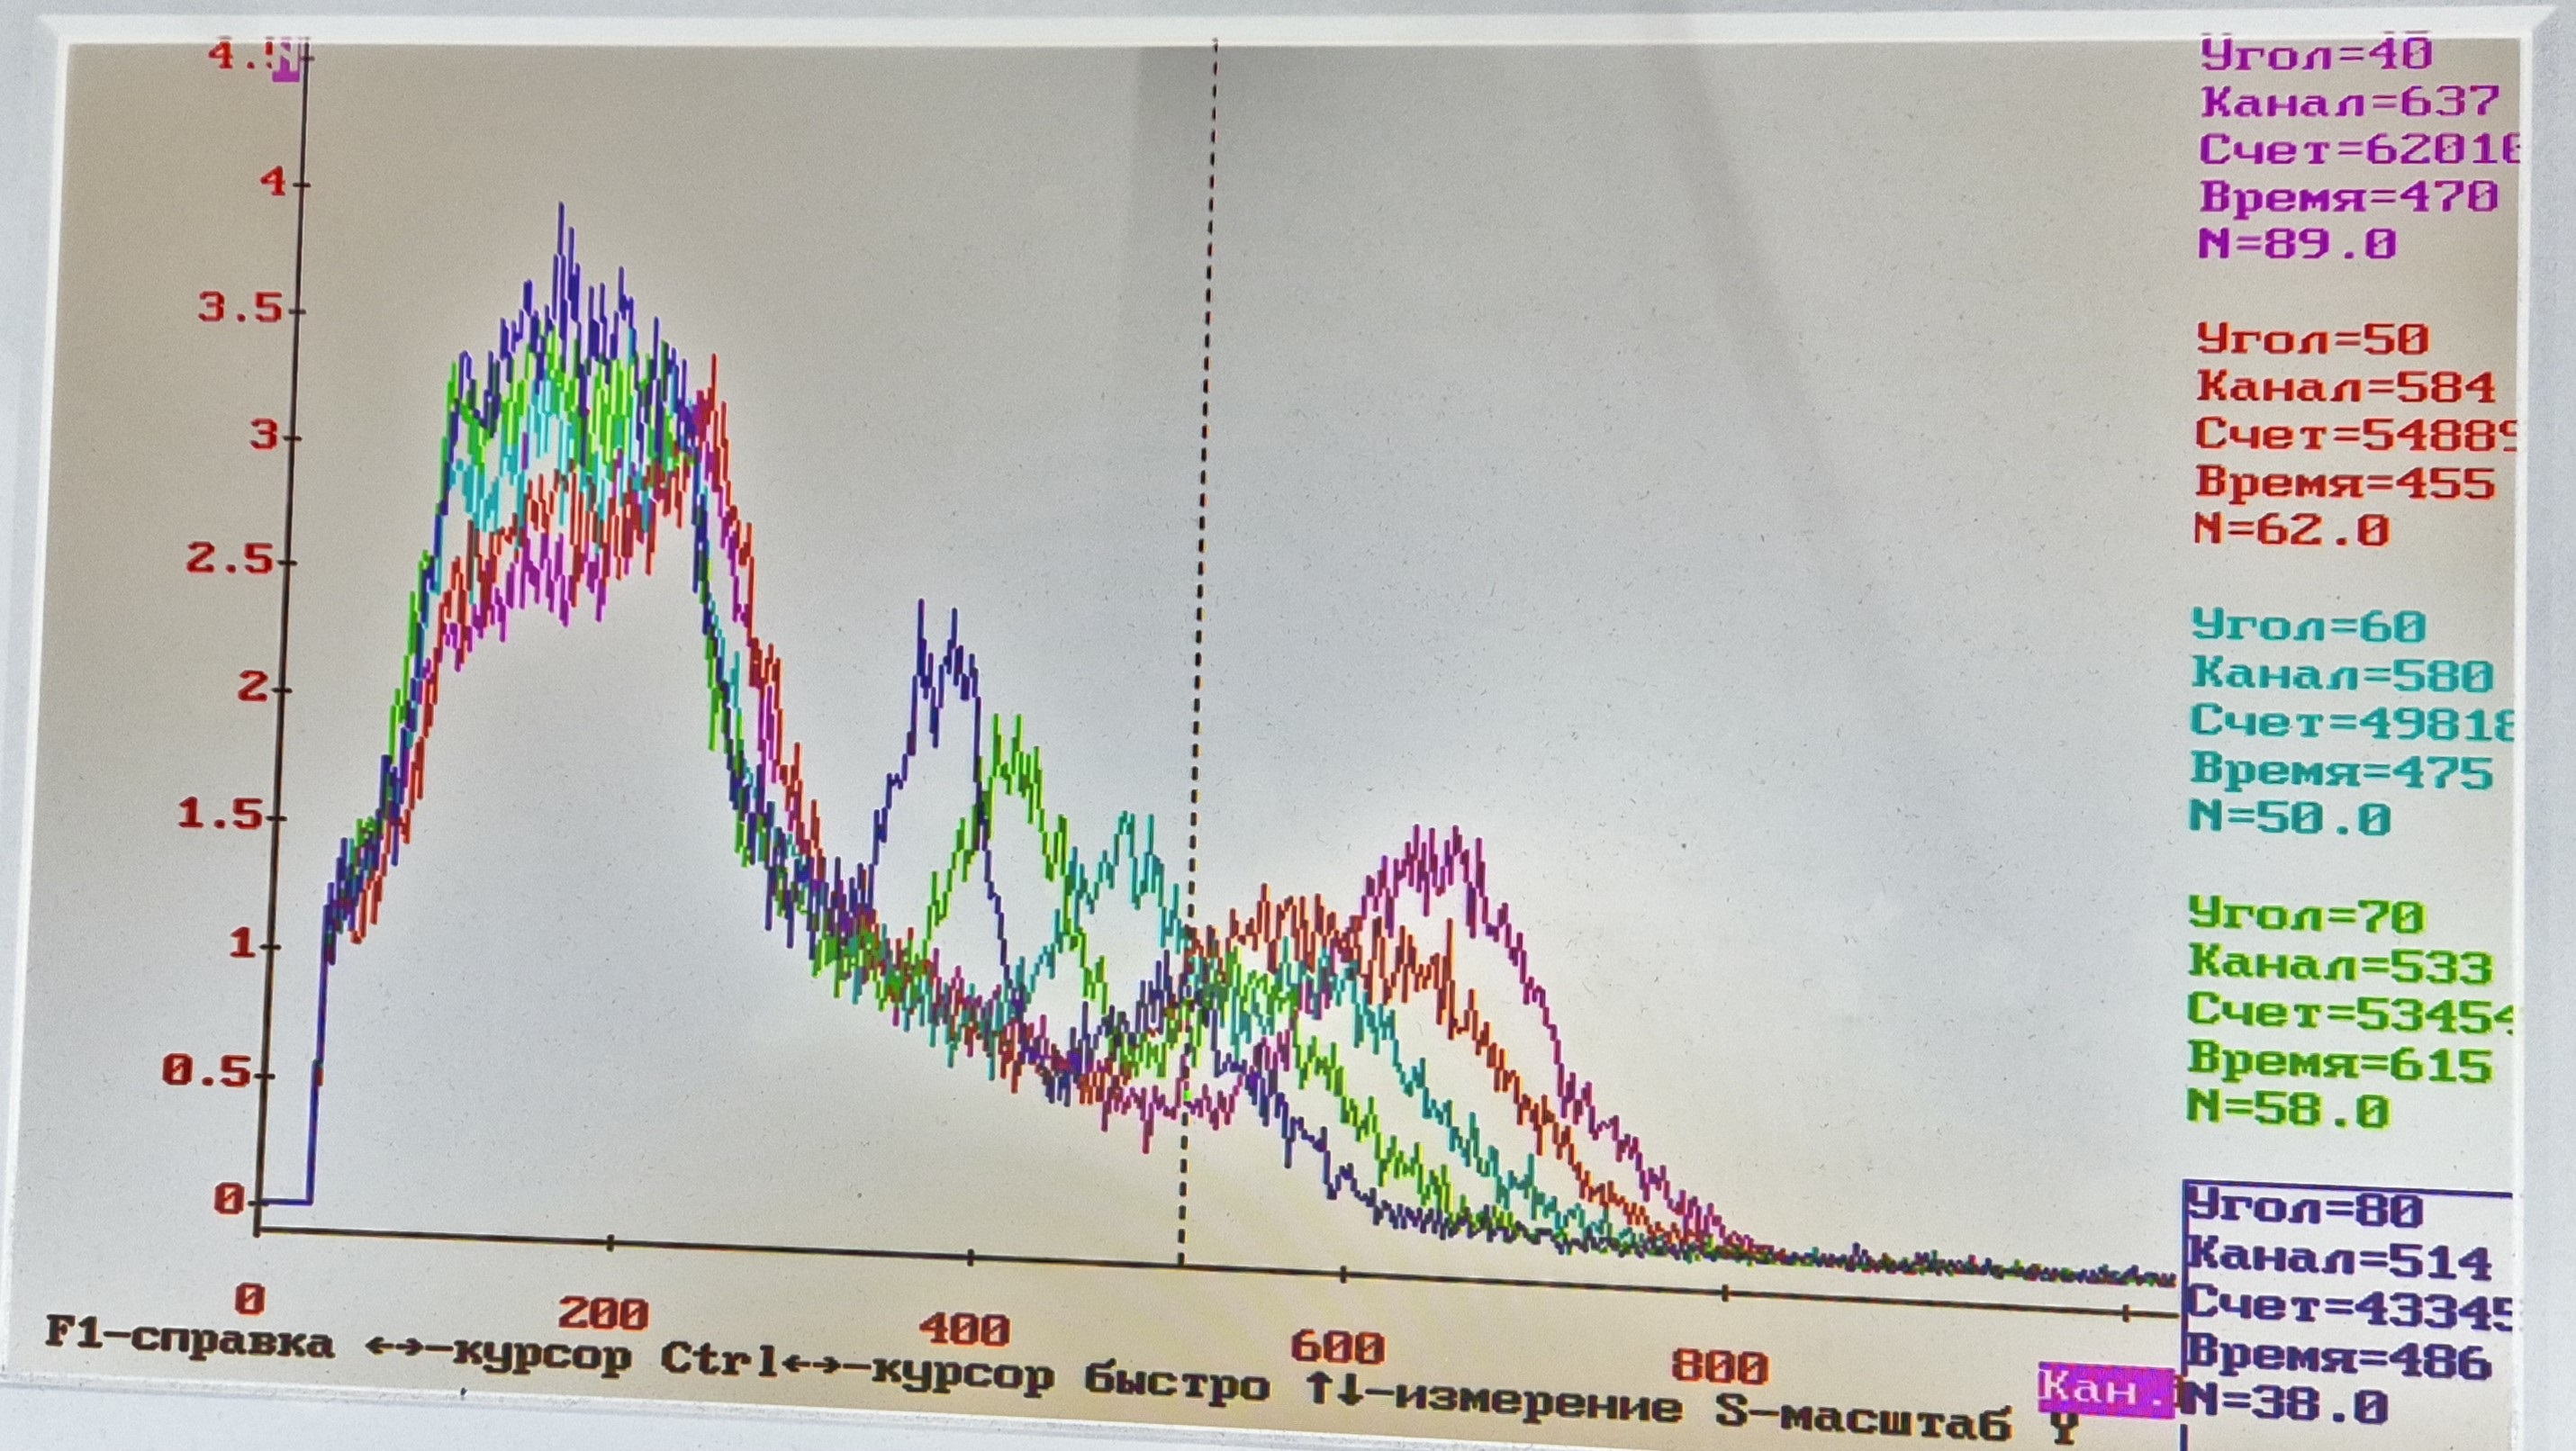
\includegraphics[width=0.85\linewidth]{../images/512-4}
\end{figure}

\begin{figure}[H]
\centering
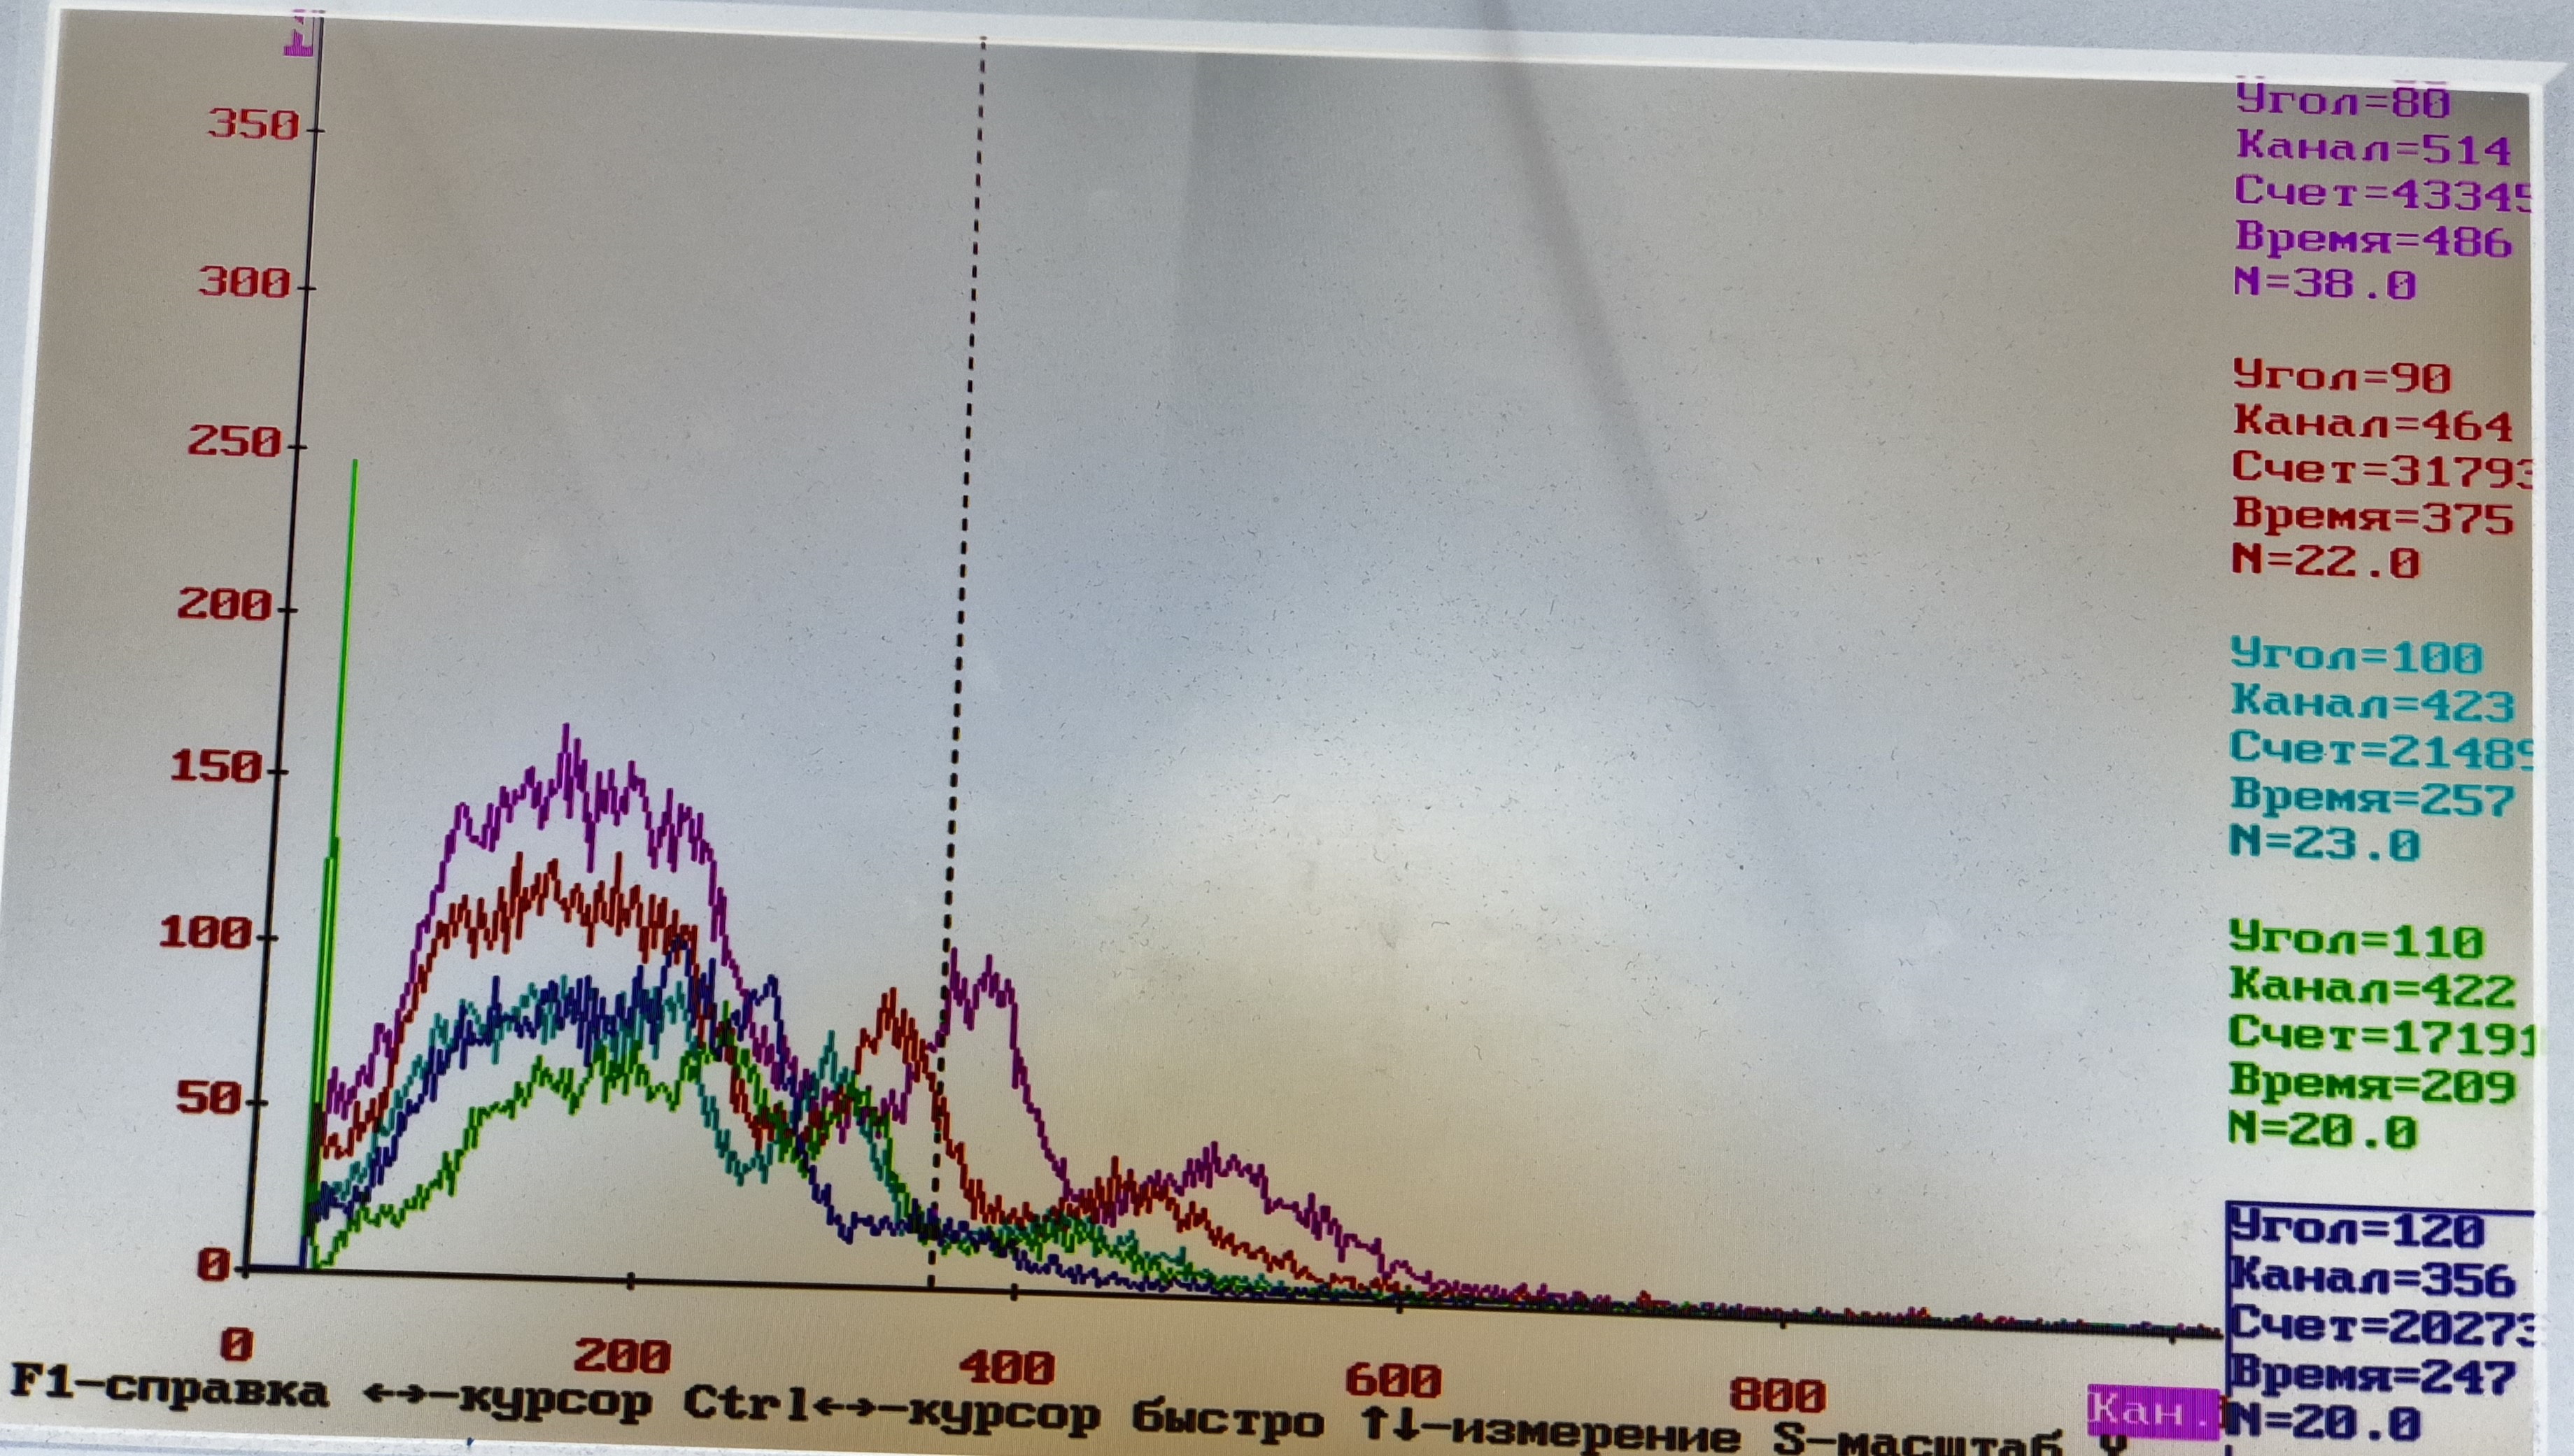
\includegraphics[width=0.85\linewidth]{../images/512-5}
\end{figure}

\newpage

\end{enumerate}

\section{Обработка результатов}

\begin{enumerate}

\item На каждом из полученных спектров определим положение фотопика. Полученные данные занесем в таблицу.

\begin{table}[H]
\centering
\begin{tabular}{|c|c|c|c|c|c|}
\hline
$\theta,\ ^\circ$  & N   & $\theta,\ ^\circ$  & N   & $\theta,\ ^\circ$   & N   \\ \hline
0  & 829 & 50 & 584 & 100 & 297 \\
10 & 847 & 60 & 480 & 110 & 313 \\
20 & 817 & 70 & 410 & 120 & 349 \\
30 & 689 & 80 & 378 &     &     \\
40 & 637 & 90 & 326 &     &     \\ \hline
\end{tabular}
\end{table}

\item Погрешность определения угла равна линейному углу, под которым виден детектор диаметром $d$ на расстоянии $l$ от источника: $\sigma_\theta=d/2l\approx4.5^\circ$. Погрешность  определения номера канала оценим по размеру плато фотопика.

\item Нанесем полученные точки вместе с их погрешностями на график в осях ($1-\cos{\theta}$) и $1/N(\theta)$. Проведем через точки прямую, заданную уравнением $y=k(x-x_0)$.

\begin{figure}[H]
\centering
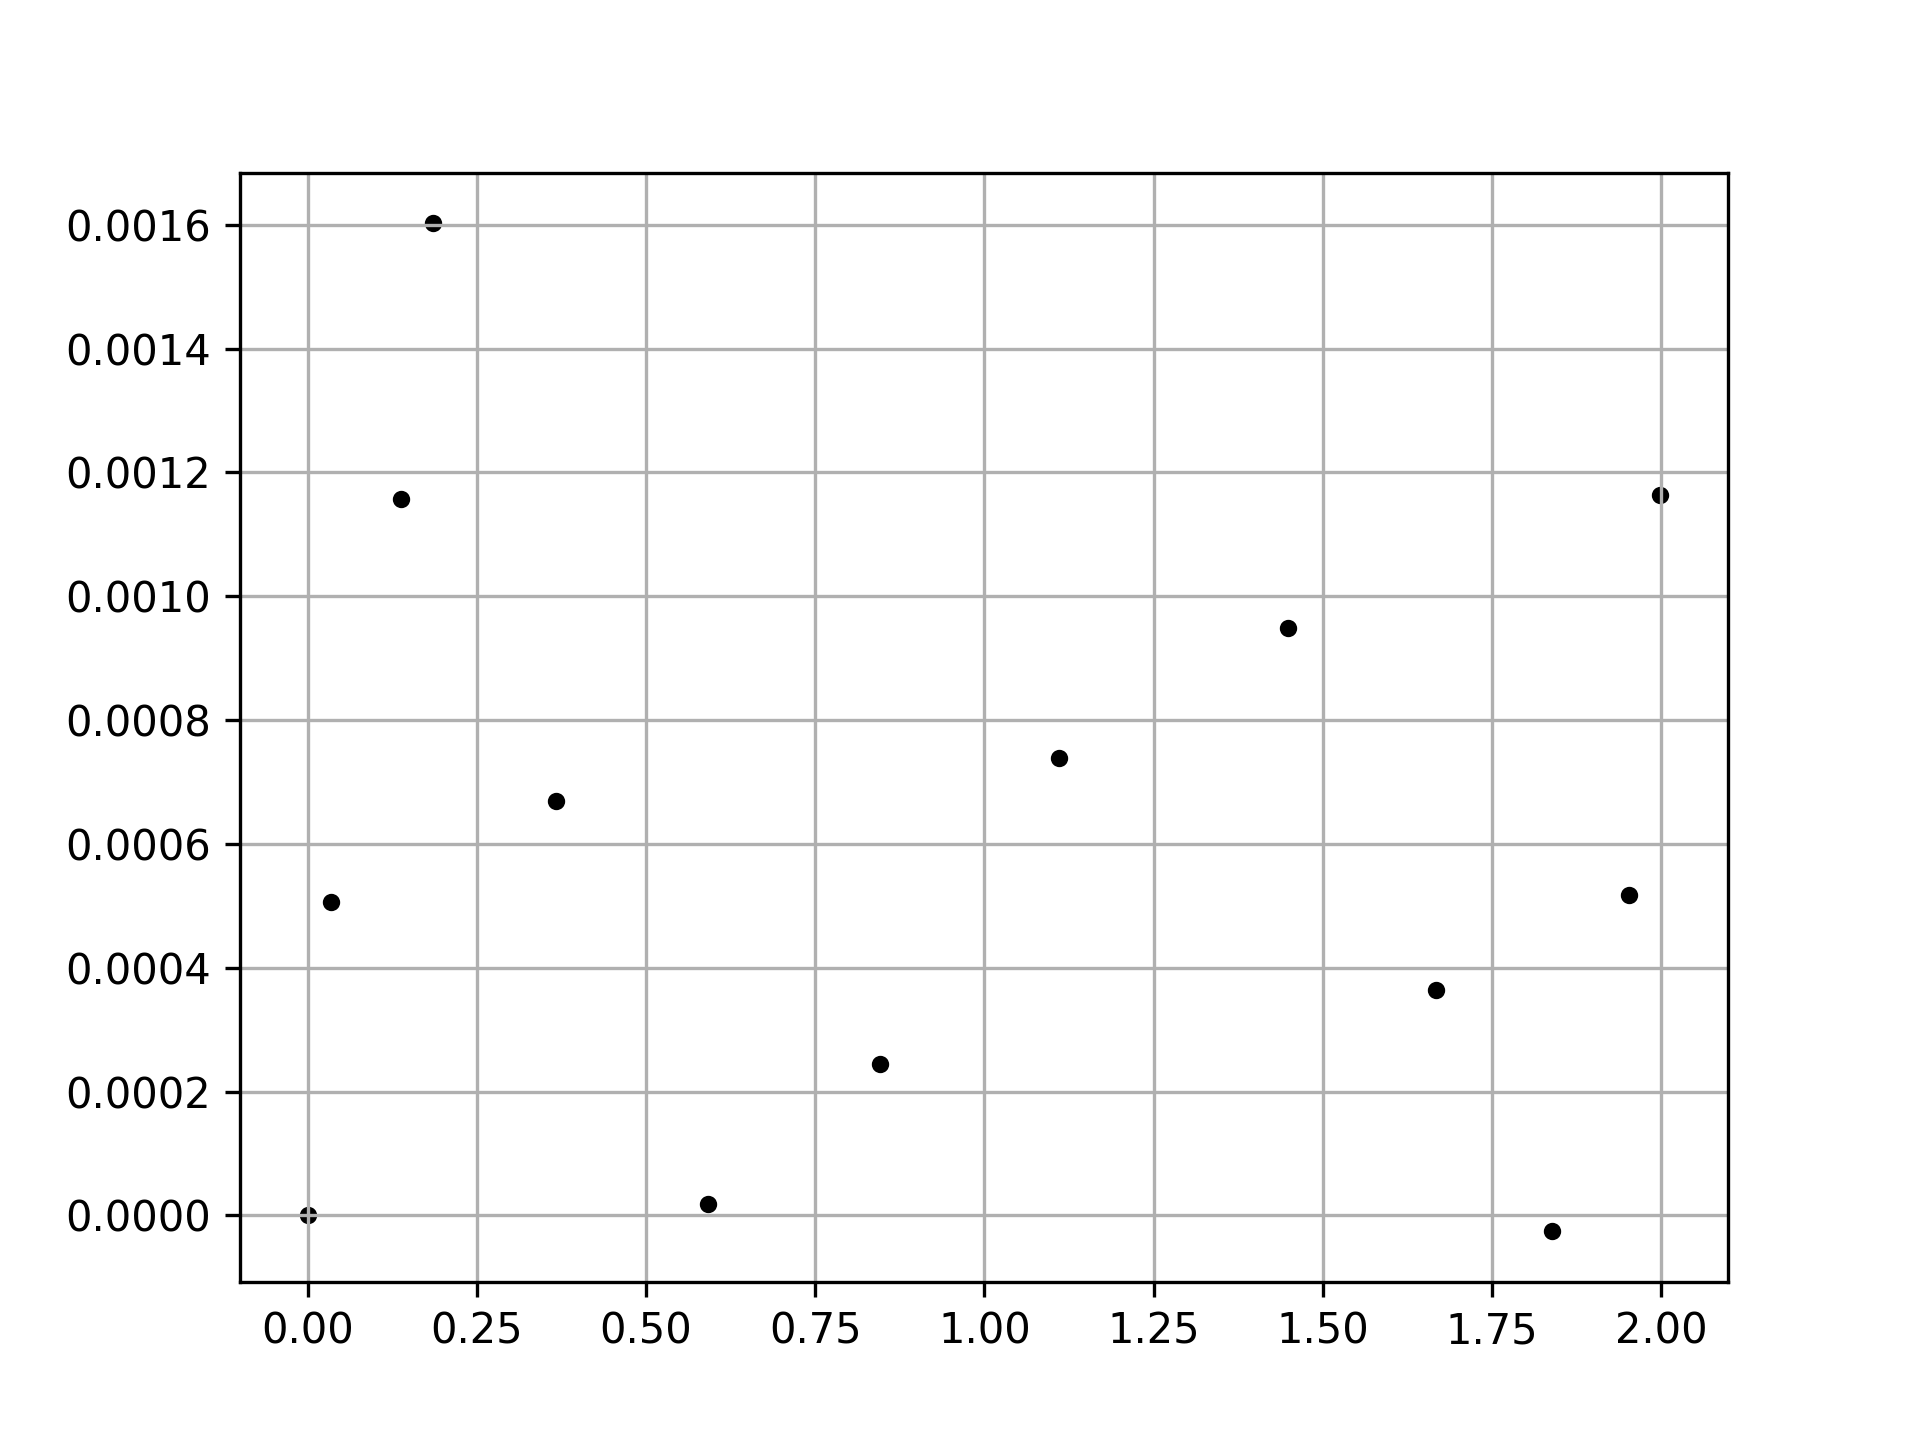
\includegraphics[width=0.7\linewidth]{../images/512-2}
\caption{График зависимости $1/N$ от ($1-\cos{\theta}$)}
\end{figure}

Выбор данных и осей и параметризации мотивирован тем, что зависимость

\[\frac{1}{E}-\frac{1}{E_0}=\frac{1}{mc^2}(1-\cos{\theta})\]

можно представить в виде

\[\frac{1}{N}=\frac{A}{mc^2}(1-\cos{\theta}+\frac{mc^2}{E_0})\text{,}\]

где $A=E/N$ -- коэффициент пропорциональности между $E$ и $N$, $E_0=662\ кэВ$ -- энергия $\gamma$-квантов, испускаемых $^{137}Cs$.

Таким образом из аппроксимации ($x_0=-0.64\pm0.10$ -- с учетом погрешности вдоль оси абсцисс) можно получить искомую энергию покоя электрона:

\[mc^2=-E_0 x_0=(420\pm70)\ кэВ\text{,}\]

что довольно близко к истинному значению $E_{покоя,\ e}=511\ кэВ$.

\end{enumerate}

\end{document}